\subsection*{Anwendungen in Branchen}
Das generative Design nimmt Einfluss in vielen verschiedenen Branchen. Darunterfallen Architektur, Automobilindustrie, Mode und Textilien, Produktgestaltung, Kunst und Design, Film und Animation, Werbung und Marketing, Spieleentwicklung, Medizin und Gesundheitswesen, Ingenieurwesen und Fertigung. Hier wird auf 3 genauer eingegangen.
Architektur: Generatives Design wird in der Architektur eingesetzt, um Gebäudestrukturen zu entwerfen. Durch die Verwendung von algorithmischen Methoden und parametrischen Modellen können Architekten komplexe und effiziente Konzepte entwickeln. Das Generative Design beeinflusst hier Parameter wie Materialverbrauch, Energieeffizienz und Raumoptimierung. 

Produktgestaltung: In diesem Bereich eröffnet das generative Design neue Möglichkeiten zur Entwicklung maßgeschneiderter und funktional optimierte Produkte. Durch den Einsatz von Algorithmen und automatisierten Prozessen können Designer Variationen von Produkten generieren und diese an individuelle Kundenanforderungen anpassen. So können einzigartige Produkte mit verbesserten Leistungsmerkmalen geschaffen werden. 

Automobilindustrie: In der Automobilindustrie wird das Generative Design verwendet, um leichtere und dennoch stabile Fahrzeugkomponenten zu entwickeln. Durch die Integration von algorithmischen Optimierungsmethoden können Ingenieure komplexe Strukturen gestalten, die mit herkömmlichen Ansätzen schwer umzusetzen wären. Das Ergebnis sind Fahrzeugkomponenten, die Gewicht einsparen und dadurch die Fahrzeugleistung verbessern. Selbes gilt für Aerodynamik und Festigkeit. \autocite*{8} \autocite{9}
\subsection*{Generativ Design Software von Autodesk und Ablauf}

Generative Design \ac*{gD} Tools werden zunehmend in verschiedenen technischen Bereichen eingesetzt. Dabei handelt es sich um Software, die verschiedene Ansätze verwenden um Designprobleme/-anforderungen zu lösen. Ein Unternehmen, das sich stark auf die Entwicklung solcher \ac*{gD}-Tools und deren Integration in herkömmliche \ac*{CAD}-Umgebungen konzentriert hat, ist Autodesk. Autodesk hat das Projekt "Dreamcatcher" gestartet, dass sich seit 2014 der Entwicklung von \ac*{gD}-Tools widmet. Nach fünf Jahren Entwicklung wurde die erste Version der kommerziellen \ac*{gD}-Software veröffentlicht. Das \ac*{gD}-Tool von Autodesk heißt Generative Design und ist in Fusion 360, einer \ac*{CAD}-Software, integriert.
Autodesk Generative Design bietet verschiedene Phasen im Arbeitsablauf, darunter:


\begin{figure}[h]
    \begin{minipage}{0.5\textwidth}
      \centering
      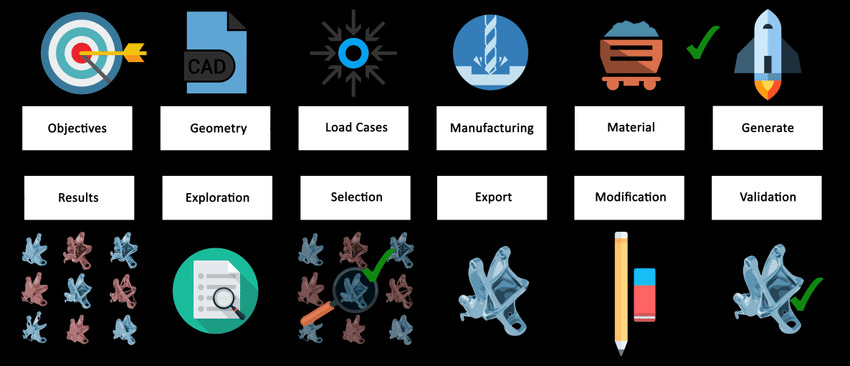
\includegraphics[width=\textwidth]{./images/Autodesk-Generative-Design-Framework.jpeg}
    \end{minipage}
    \caption{Autodesk Prozessablauf}
    \label{fig:meinbild}
  \end{figure}
  
  1.	Ziele: Der Benutzer kann zwischen zwei Optionen wählen, entweder die Masse zu minimieren oder die Steifigkeit zu maximieren. In beiden Fällen wird ein Sicherheitsfaktor benötigt. Bei Auswahl der zweiten Option muss der Anwender auch eine Zielmasse angeben, die die Optimierung erreichen soll.
  2.	Geometrie: Der Benutzer definierte die Bereiche, die von der Optimierung verschont bleiben sollen (Erhaltungsbereiche) und die Bereiche, die leer bleiben müssen (Hindernisbereich). 
  3.	Lastfälle: Generative Design unterstütz Kräfte, Druck und Lagerlast. Es kann auch die Schwerkraft berücksichtigen. Die Lasten müssen auf die vorher erstellten Erhaltungsbereiche angewandt werden. 
  4.	Fertigungsbeschränkungen: Der Benutzer kann Fertigungsbeschränkungen angeben, um die Fertigung später zu erleichtern (5-Achs-Fräsen, 4-Achs-Fräsen). Dies spart Produktionskosten ein.
  5.	Material: Generativ Design ermöglicht die Auswahl von bis zu zehn verschiedenen Materialien in einer Analyse. 
  6.	Eingabeprüfung und Berechnung: Generative Design überprüft, ob alle erforderlichen Informationen korrekt sind. Wenn ja, werden die Optimierungen auf externen Servern durchgeführt. 
  7.	Ergebnisse: Sobald die Ergebnisse auf dem lokalen Computer heruntergeladen sind, können diese Visualisiert werden. 
  8.	Exploration: Generative Design bietet eine dedizierte Umgebung mit Visualiserungswerkzeugen, um die Ergebnisse geordnet darzustellen. Das hilft bei der Identifizierung der besten Lösung.
  9.	Auswahl: Der Anwender wählt die Lösung aus, die am besten den gewünschten Anforderungen entspricht und exportiert diese.
  10.	Export: das Designt wird isoliert und für weitere Änderungen verfügbar gemacht. \ac*{CAD}-Geometrie des Teils wird in die Modellierungsumgebung von Fusion 360 importiert.
  11.	Modifikation: Nach dem Export der Lösung, muss es mit herkömmlichen \ac*{CAD}-Tools bearbeitet werden, um Fehler zu beheben.
  12.	Validierung: Die Leistungsfähigkeit der exportierten Form muss durch zusätzliche Finite-Elemente-Analysen validiert werden. \autocite*{7}

\subsection*{Generatives Design für Leichtgewicht}

Durch das generative Design lässt sich die Materialeffizienz eines Designs verbessern, während die Leistungsparameter und Funktionalitätsanforderungen erhalten bleiben. Die Software entfernt Material an Stellen, an denen es nicht benötigt wird, und strukturiert es organisch um, basierend auf Stress- und Dehnungsmustern. Dadurch kann ein generativ gestaltetes Bauteil bei gleichbleibender Funktionalität eine Materialreduktion von bis zu 80 Prozent erreichen!

\begin{figure}[h]
  \begin{minipage}{0.5\textwidth}
    \centering
    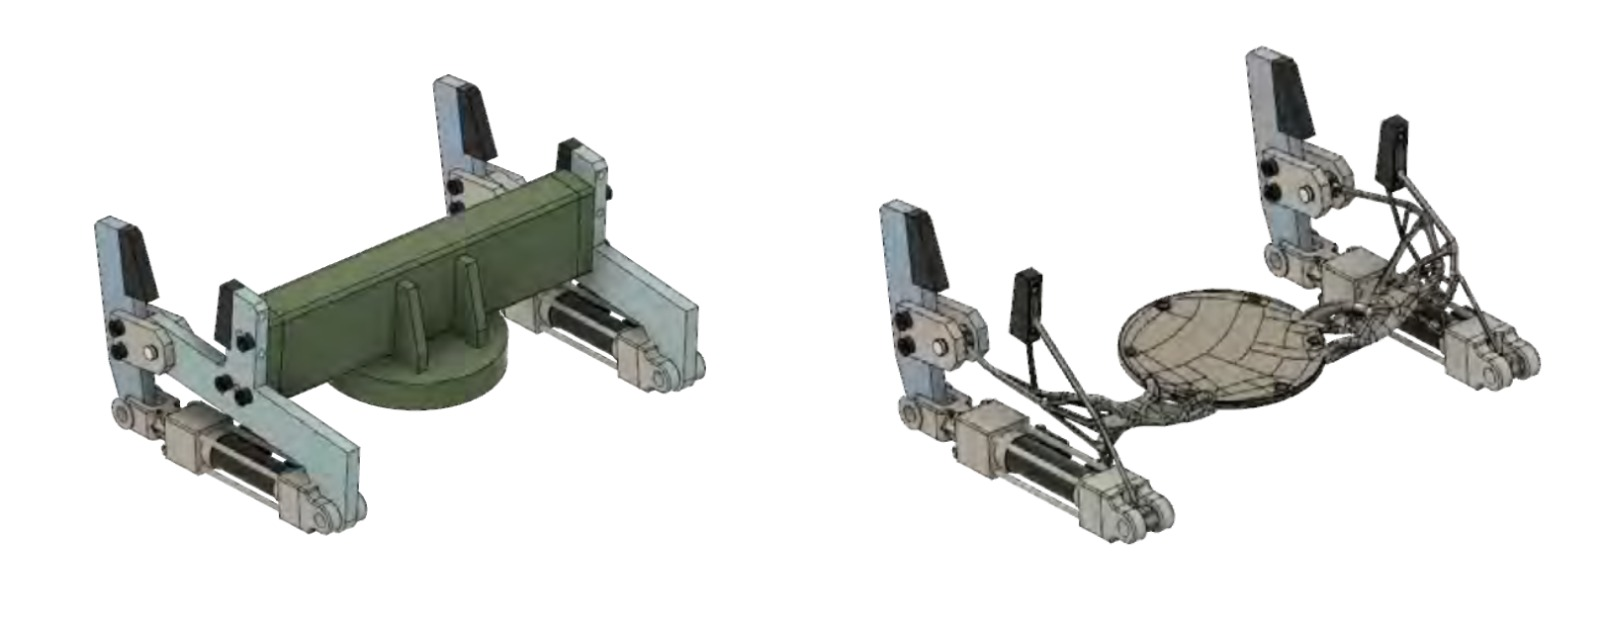
\includegraphics[width=\textwidth]{./images/WhatsApp Image 2023-06-11 at 23.48.25.jpeg}
  \end{minipage}
  \caption{Generativ Designtes Bauteil}
  \label{fig:meinbild}
\end{figure}

Die Herstellung generativ gestalteter Teile erfolgt oft durch additive Fertigung, auch bekannt als 3D-Druck. Additive Fertigung ermöglicht die effiziente Herstellung komplexer Designs, die mit herkömmlichen Verfahren schwer umsetzbar wären. Zwei 3D-Druckverfahren, Powder Bed Fusion (PBF) für Stahl und Fused Deposition Modeling (FDM) für Polycarbonat, sind die am weitesten verbreiteten.

Eine wichtige Komponente des generativen Designs ist die Software Autodesk Netfabb, die Werkzeuge zur Optimierung des 3D-Druck-Workflows bietet. Mit dieser Software können Stützstrukturen, Fütterungs- und Geschwindigkeitseinstellungen optimiert werden, um den Material- und Energieverbrauch zu minimieren.

Um die Umweltauswirkungen der generativ gestalteten Bauteile und des Herstellungsprozesses zu bewerten, wird eine umfassende Lebenszyklusanalyse (LCA) durchgeführt. Diese berücksichtigt den gesamten Lebenszyklus des Bauteils, einschließlich der Rohstoffverarbeitung, der Herstellung, der Nutzung und der Entsorgung. Die Ergebnisse zeigen, dass generativ gestaltete Teile, die mit additiven Verfahren hergestellt werden, eine geringere Umweltbelastung aufweisen als Teile, die mit herkömmlichen Verfahren gefertigt werden.

\subsection*{TestFit Plattform und Fallbeispiel in  Rio de Janeiro}

TestFit ist eine Software für generatives Design im Bauwesen. Sie wurde von der Firma TestFit Inc. entwickelt und bietet eine benutzerfreundliche Oberfläche zur Generierung von Anfangsentwürfen und zur finanziellen Machbarkeitsprüfung von Immobilienprojekten.

Die Software ist in vier Hauptbereiche unterteilt (\autoref{fig:software}). Im oberen linken Bereich können verschiedene Projekte verwaltet und deren Eigenschaften wie städtebauliche Bedingungen, finanzielle Daten, Gebäude- und Einheitenmerkmale angepasst werden. Der untere linke Bereich ermöglicht detaillierte Bearbeitungen wie die Änderung der Gebäudehöhe oder der allgemeinen Gebäudekonfiguration.

Der große obere rechte Bereich der Software bietet verschiedene grafische Ressourcen wie 3D-Visualisierungen und 2D-Pläne, um die generierten Entwürfe zu visualisieren. Der untere rechte Bereich zeigt die generierten Lösungen an, wie die Anzahl der Einheiten pro Fläche und die finanziellen Ergebnisse des Projekts. Es können auch Vergleiche zwischen verschiedenen Entwurfsalternativen durchgeführt werden.

TestFit zeichnet sich durch seine generative Fähigkeit aus, mit der es anhand vorgegebener Parameter optimale Lösungen generiert. Es ermöglicht die Manipulation einer Vielzahl von Baumerkmalen und bietet eine schnelle Algorithmusgenerierung. Die Software unterstützt auch die Erstellung, Bearbeitung und den Vergleich von verschiedenen Entwurfsalternativen.

\begin{figure}[h]
  \begin{minipage}{0.5\textwidth}
    \centering
    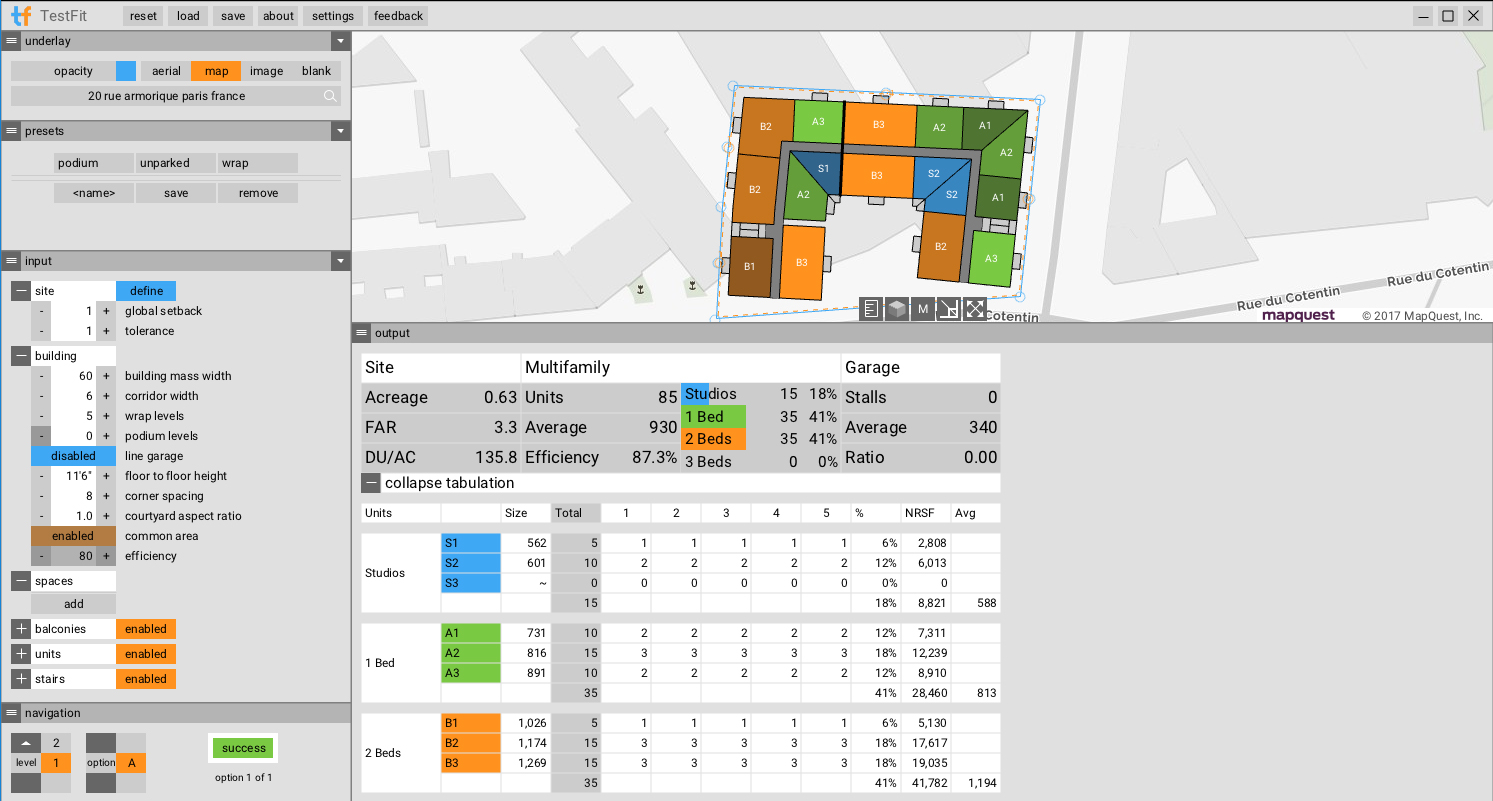
\includegraphics[width=\textwidth]{./images/UnitsData.jpg}
  \end{minipage}
  \caption{TestFit Software}
  \label{fig:software}
\end{figure}

Fallstudie in Rio de Janeiro, bei der das generative Design zur Optimierung der Raumplanung und des Wohnungsbaus eingesetzt wurde. Das Ziel war es, mithilfe einer speziellen Software maximale Raumnutzung und eine vorgegebene Anzahl von Wohnungen mit bestimmten Größen und Anteilen zu erreichen.

Zunächst wurden bestimmte Kriterien definiert, um einen geeigneten Standort in Rio de Janeiro auszuwählen. Es wurde ein Bereich im Stadtteil Santo Cristo identifiziert, der die erforderlichen Voraussetzungen erfüllte, wie ausreichende Größe und bekannte Zonierungsbeschränkungen. Dieser Bereich wurde als "besonderes Gebiet von städtischem Interesse" eingestuft und bot steuerliche Vorteile für den Wohnungsbau.

Die generative Design-Software wurde verwendet, um Lösungen für den Wohnungsbau in diesem Gebiet zu generieren. Die Software ermöglichte die Eingabe verschiedener Parameter wie Gebäudehöhe, Gebäudekonfiguration, Flächennutzung und Wohnungsgrößen. Anhand dieser Parameter generierte die Software automatisch verschiedene Lösungsalternativen.

Zur Bewertung der generierten Lösungen wurden neun Parameter festgelegt, darunter die Gesamtbaufläche, die Anzahl der Einheiten, die durchschnittliche Wohnungsgröße und die Flächenproportionen der verschiedenen Wohnungstypen. Die Ergebnisse wurden analysiert, um festzustellen, inwieweit die Ziele der Maximierung der Raumnutzung und der Generierung der gewünschten Wohnungsanzahl und -größen erreicht wurden.

Es wurden mehrere Iterationen des generativen Designprozesses durchgeführt, um die Lösungen kontinuierlich zu verbessern. Dabei wurden verschiedene Gebäudekonfigurationen und -layouts ausprobiert, um die gewünschten Ergebnisse zu erzielen.



\subsection*{Fallbeispiel Heydar Aliyev Centre}
Für das Heydar Aliyev Centre wurde die Software Rhino 3D verwendet. Rhino ist eine 3D-Modellierungssoftware, die sich durch ihre Vielseitigkeit und ihre Fähigkeit zur Generierung komplexer Formen auszeichnet.

\begin{figure}[h]
    \begin{minipage}{0.5\textwidth}
      \centering
      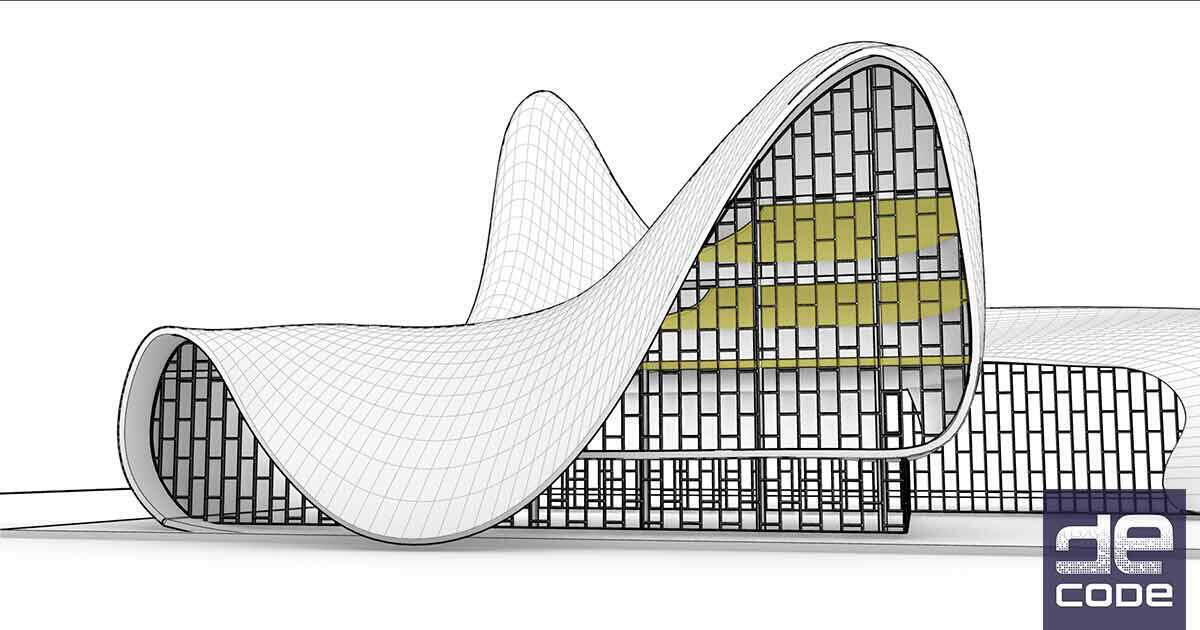
\includegraphics[width=\textwidth]{./images/DE_Rh_lvl1_baku.jpg}
    \end{minipage}
    \caption{Heydar Aliyev Centre}
    \label{fig:centre}
  \end{figure}

Das Heydar Aliyev Centre in Baku, Aserbaidschan ist ein architektonisches Meisterwerk von Zaha Hadid (\autoref{fig:centre}). Es vereint Kunst, Kultur und Geschichte und beeindruckt mit seinen fließenden Formen und der innovativen Raumgestaltung. 
Bei der Gestaltung wurde generatives Design verwendet, um die organischen Kurven und fließenden Formen des Gebäudes zu schaffen. Das Design-Team legte verschiedene Parameter und Kriterien fest wie beispielsweise Raumfunktionen, Nutzungsanforderungen, ästhetische Präferenzen und strukturelle Stabilität. 
Basierend auf diesen Parametern konnte das System unzählige mögliche Designs generieren. Dabei wurden Aspekte wie räumliche Effizienz, natürliche Belichtung, Zugänglichkeit und visuelle Harmonie berücksichtigt. Das generative Design ermöglichte es den Architekten, schnell eine Vielzahl von Variationen zu erforschen und diejenige auszuwählen, die am besten den Anforderungen entsprachen. 
Das Ergebnis ist ein einzigartiges und faszinierende architektonisches Konzept, das ohne den Einsatz von generativem Design vermutlich nicht realisierbar gewesen wäre. Dieses Bauwerk zeigt, wie computergesteuerte Designmethoden neue Horizonte eröffnen. 
Generatives Design hat nicht nur zur Schaffung eines ikonischen Gebäudes beigetragen, sondern es hat auch die Effizienz und Nachhaltigkeit des Designs verbessert. Durch die Berücksichtigung von Faktoren wie Energieeffizienz und optimierte Raumnutzung konnte das Heydar Aliyev Centre eine umweltfreundliche und ressourcenschonende Architektur realisieren. \autocite*{5}
